67. $y=-\cfrac{4|x+2|}{x^2+2x}=-\cfrac{4|x+2|}{x(x+2)}=\begin{cases} -\cfrac{4}{x},\ x>-2,\\ \cfrac{4}{x},\ x<-2.\end{cases}$
$$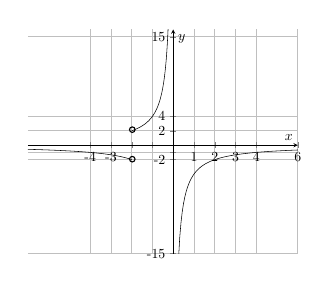
\begin{tikzpicture}[scale=0.5]
\begin{axis}[
    axis lines = middle,
    grid=major,
    legend pos={south west},
    xlabel = {$x$},
    %xlabel style={below right},
    ylabel = {$y$},
    ymin=-15,
    ymax=16,
    xmin=-7,
    xmax=6,
    xtick={-4,-3,-2,-1,1,2,3,4,6},
    xticklabels={-4,-3,$ $,$ $,1,2,3,4,6},
    ytick={-15, -2,-1,2,4,15},
    yticklabels={-15, -2,$ $,2,4,15},
                  ]
	\addplot[domain=-7:-2, samples=100, color=black] {(4/x)};
    \addplot[domain=-2:-0.01, samples=100, color=black] {-(4/x)};
    \addplot[domain=0.01:6, samples=100, color=black] {-(4/x)};
    %\addplot[domain=2.01:6, samples=100, color=black] {2/(2-x)};
   % \addplot[domain=-3:3, samples=100, color=black] {-x};
     %\addlegendentry{$\text{Рис. 1}$};
\end{axis}
\draw (2.65,3.15) circle (2pt);
\draw (2.65,2.4) circle (2pt);
\end{tikzpicture}$$
По графику определим $m\in(-\infty;-2]\cup(2;+\infty).$\\
